\chapter{Evaluating Word Vectors}\label{ch:eval}

\section{Evaluation Metrics}

We need to measure the distance between vectors to define similarity between word vectors and therefore analogies between words:

\begin{itemize}
  \item 
    \textbf{Euclidean Distance}: 
    \[
      d_\mathrm{euclid}(x,y) = \sqrt{\sum\limits_{i=1}^n(x_i - y_i)^2}
    \]

  \item 
    \textbf{Cosine Distance}
    \[
      d_\mathrm{cosine}(x,y) = 1 - \mathrm{cos}(\angle (x, y)) = 
      1 - \underbrace{\frac{\langle x,y\rangle}{\|x\|_2\|y\|_2}}_{\mathrm{Cosine\ Similarity}}
    \]
\end{itemize}

In general we could use every metric to evaluate the model. But the 
cosine similarity is more robust in terms of curse of dimensionality.

\begin{figure}[!h]
\centering
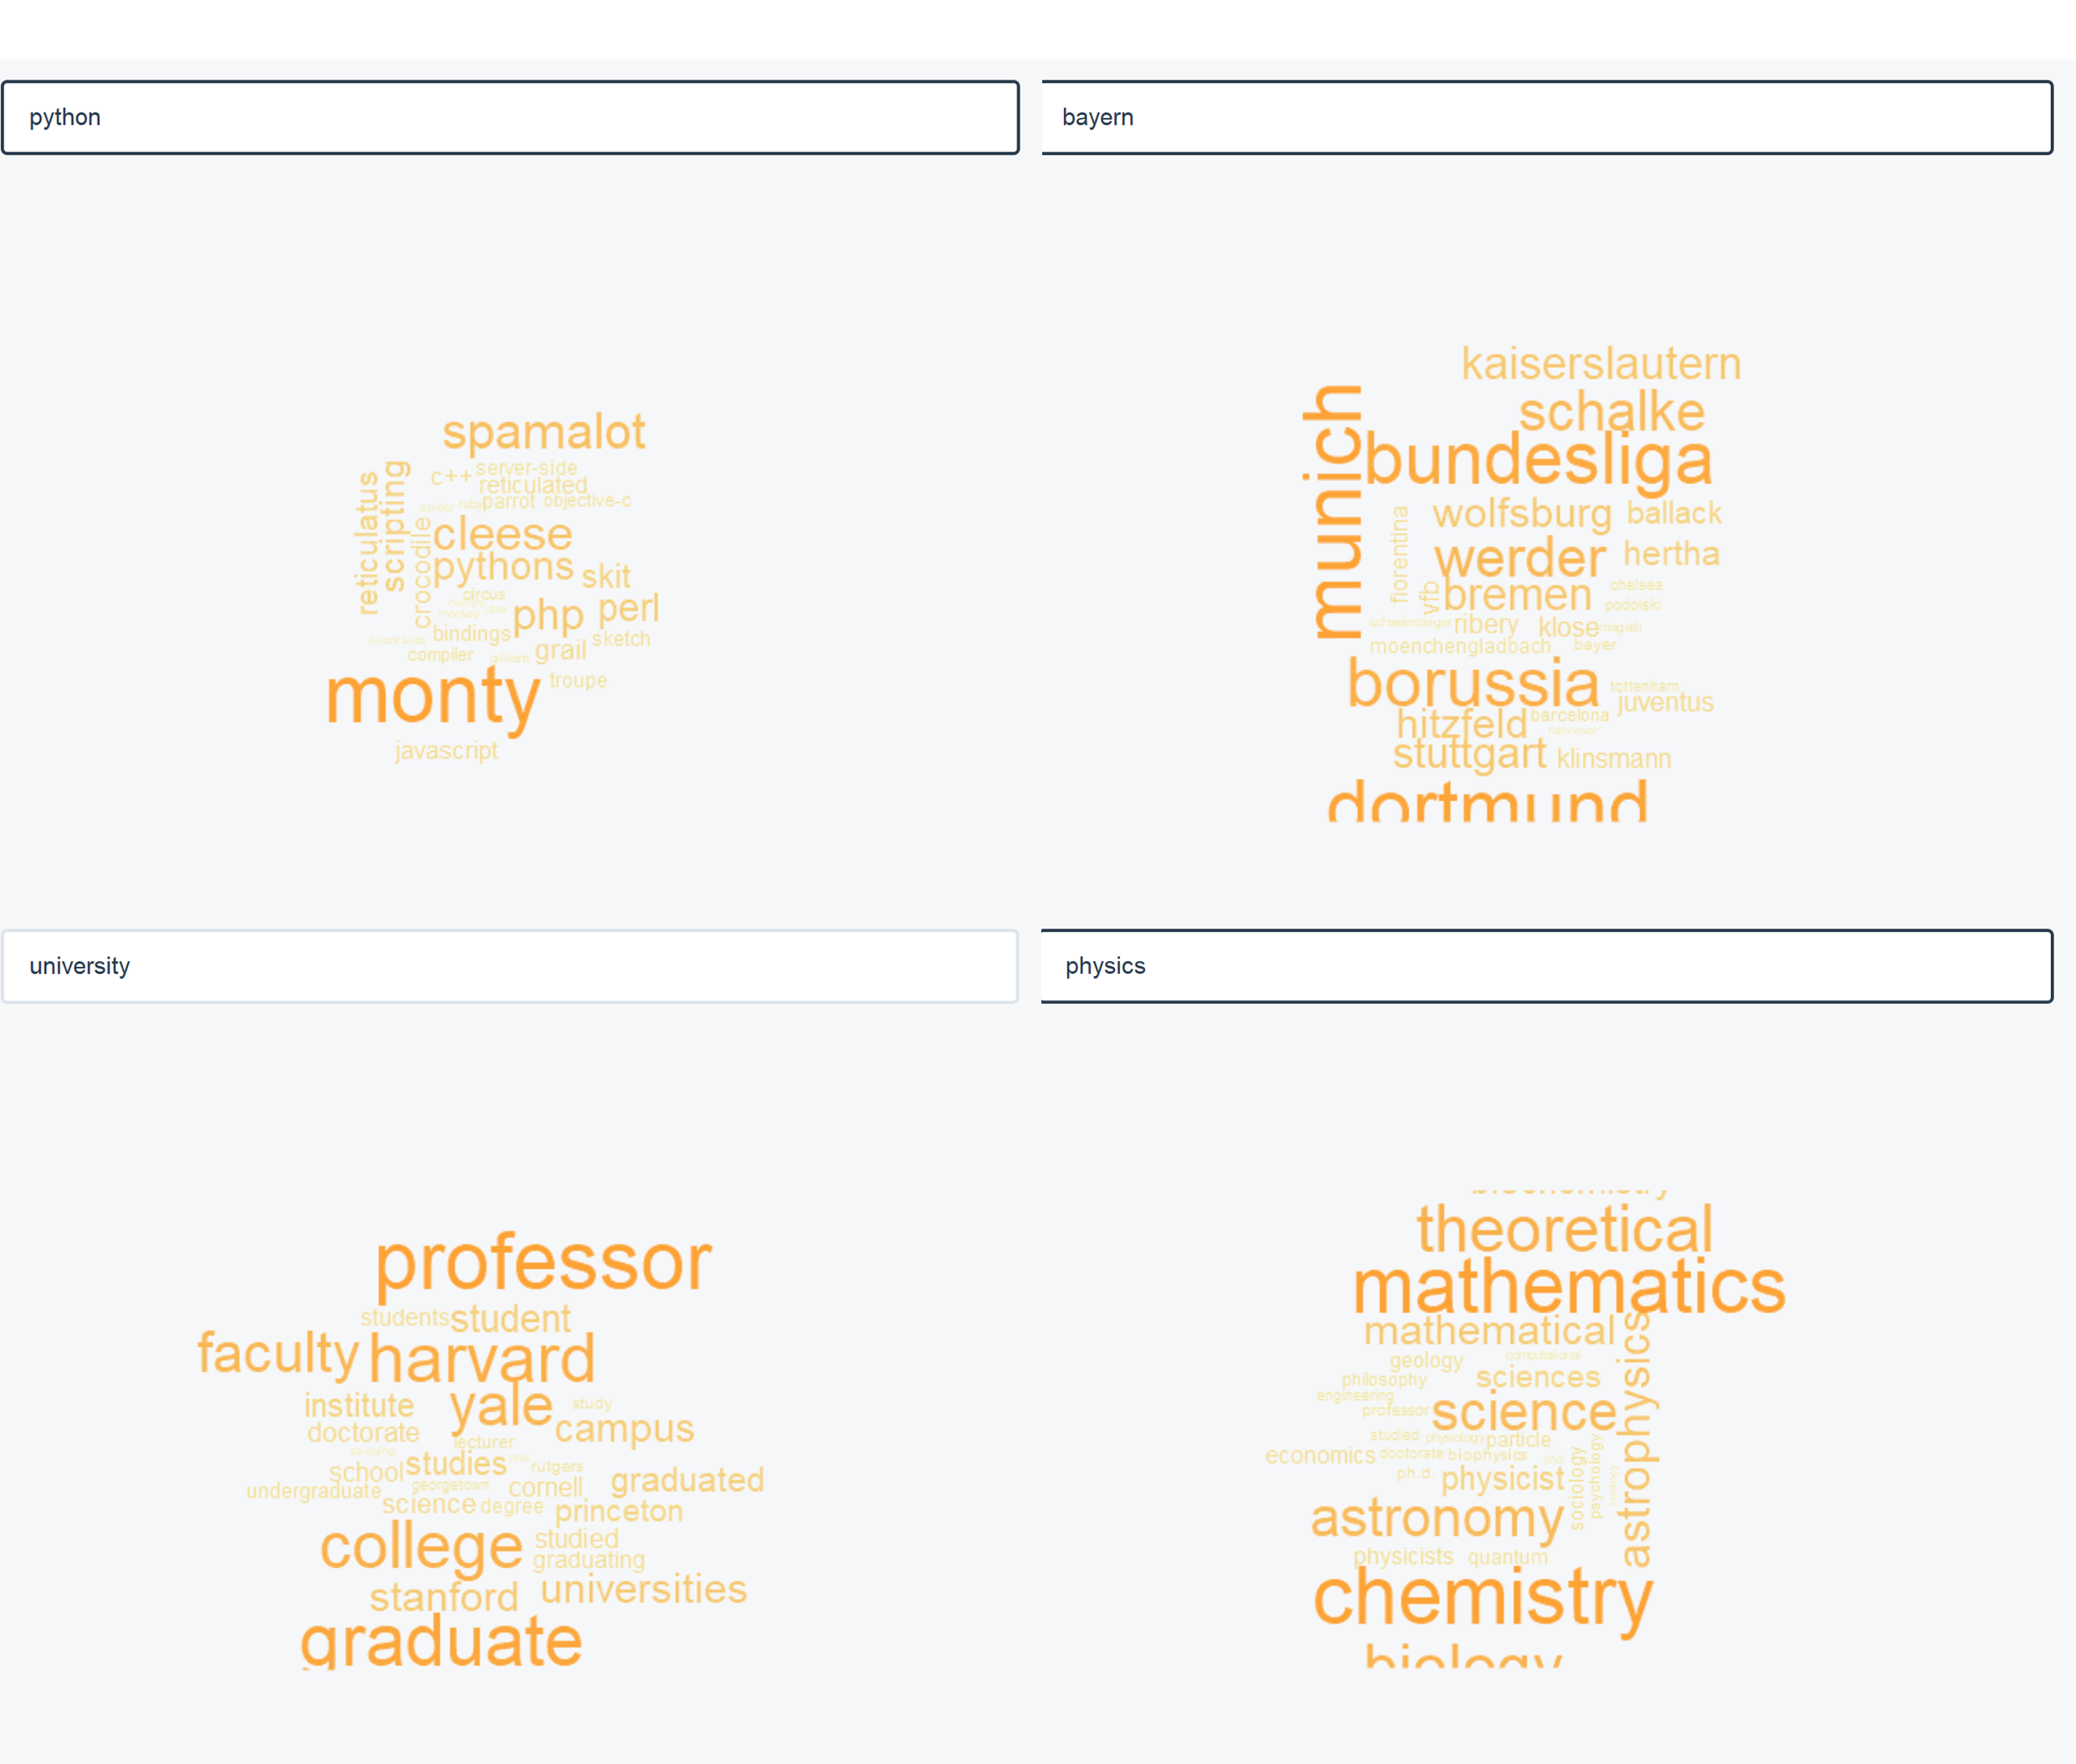
\includegraphics[scale=0.5]{images/word_clouds.png} 
\caption[Different word clouds illustrating similarities.]{Different word clouds for the words python, bayern, university and physics. The bigger the words, the smaller the cosine distance. The images are taken from an shiny application programmed for this seminar using pre trained word vectors from \cite{pennington2014glove} using the wikipedia dump (see section \ref{ch:data}).}
\label{fig:wc}
\end{figure}

\section{p-Norm in high Dimensions}

\cite{aggarwal2001surprising} have shown, that in high dimensions the ratio of the 
maximal norm divided by the minimal norm of $n$ points $x_1, \dots, x_n$
which are randomly drawn converges in probability to 1 for increasing
dimension $d$:
\[
\underset{{d\rightarrow\infty}}{\mathrm{p~lim}}\ \frac{\mathrm{max}_k \|x_k\|_2}{\mathrm{min}_k \|x_k\|_2} = 1
\]
This means if we use the euclidean norm, in high dimensions points are almost surely concentrated on the surface of a hyper sphere. The same holds for every $p$-Norm.
Figure \ref{fig:p-norm} shows an simulation of the $p$-Norm in high dimension.


\begin{figure}[!h]
\centering
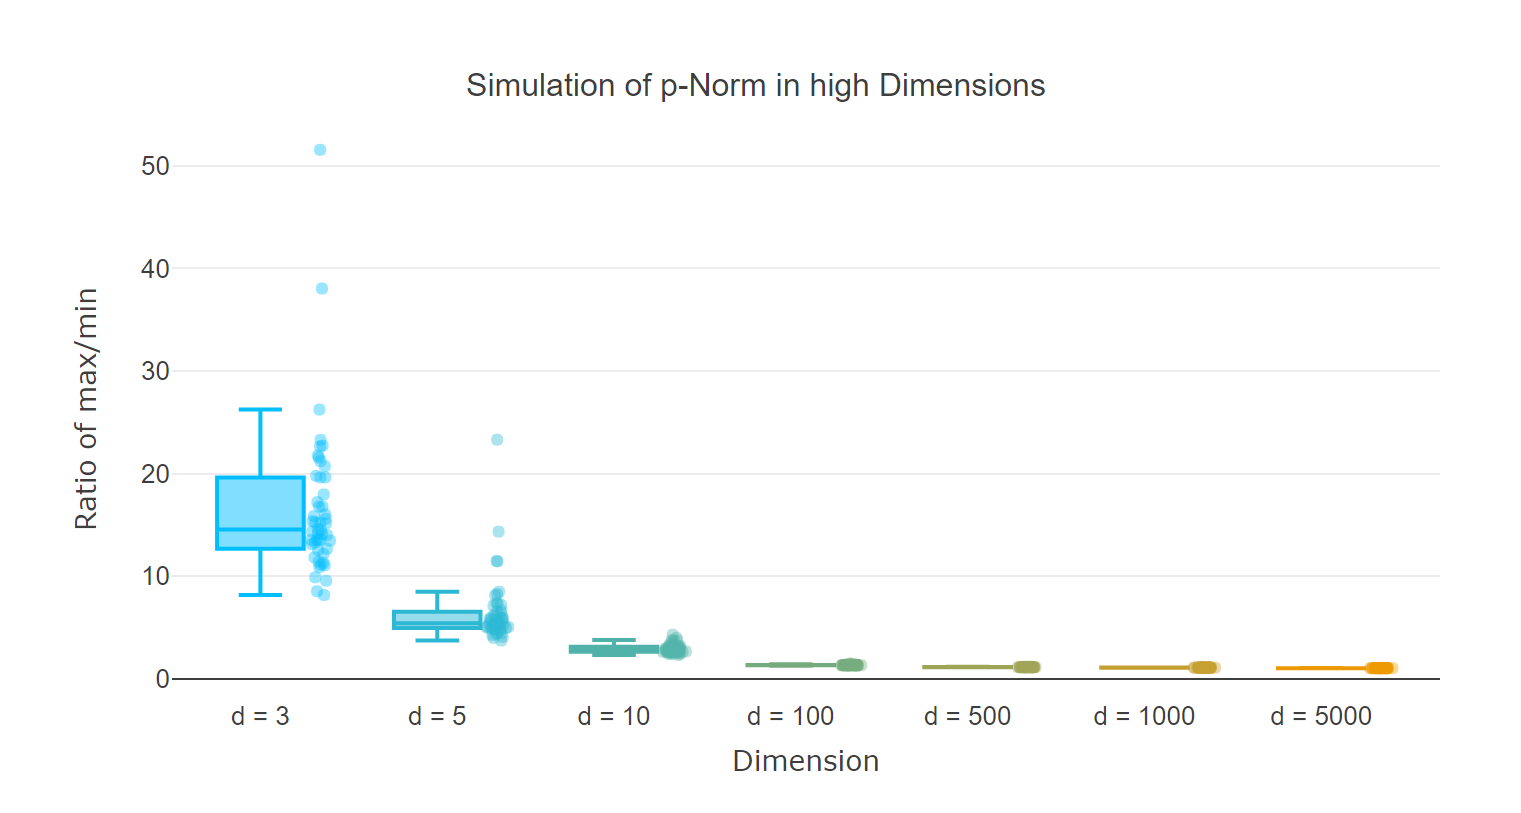
\includegraphics[width=0.9\textwidth]{images/p_norm_hd.png} 
\caption[Curse of dimensionality simulation.]{Simulating the curse of dimensionality
         by drawing 100 points of a uniform distribution on a hypercube and 
         calculating the ratio of the longest and the shortest vector. This is 
         repeated 50 times for each of the dimensions 3, 5, 10, 100, 500, 
         1000 and 5000.}
\label{fig:p-norm}
\end{figure}


\section{Semantic and Analogies}\label{sec:sem-ana}

One thing we can do now is to ask for semantic analogies between words. 
Something like:

\begin{align*}
\mathrm{paris\ behaves\ to\ france\ }&\mathrm{like\ berlin\ to\ ?} \\
\mathrm{animal\ behaves\ to\ animals\ }&\mathrm{like\ people\ to\ ?} \\
\mathrm{i\ behaves\ to\ j\ }&\mathrm{like\ k\ to\ l} 
\end{align*}

Therefore, we have $3$ given word vectors $w_i$, $w_j$ and $w_k$. To get the 
desired fourth word $l$ we use the linearity of the word vector space:
\[
w_l \approx w_j - w_i + w_k
\]
We can explain this linear combination by remembering the introduction where
we explained, that the context of words (e.~g.~is capital) is memorised within
the difference of words. We now add this context to the desired word to obtain
the corresponding context word. Furthermore, we obtain $\widehat{l}$ from our 
model and a given metric $d(w_i, w_j)$ (mostly $d = d_\mathrm{cosine}$) by
computing:
\[
\widehat{l} = \underset{l \in V}{\mathrm{arg~min}}\ d(w_j - w_i + w_k, w_l)
\]


\section{Questions Words File}

To evaluate trained word vectors, \cite{mikolov2013efficient} provide a word
similarity task. This task is given within a question words file which
contains about 19544 semantic analogies. The following list shows the first
10 tasks:

\begin{Shaded}
\begin{verbatim}
: capital-common-countries
Athens Greece Baghdad Iraq
Athens Greece Bangkok Thailand
Athens Greece Beijing China
Athens Greece Berlin Germany
Athens Greece Bern Switzerland
Athens Greece Cairo Egypt
Athens Greece Canberra Australia
Athens Greece Hanoi Vietnam
Athens Greece Havana Cuba
Athens Greece Helsinki Finland
\end{verbatim}
\end{Shaded}

Basically, this 19544 tasks are separated into 14 categories. Table \ref{tab:qwfile}
shows all the categories, how much tasks each category has and an example for each
category.

\begin{center}
\begin{table}[!h]
\begin{tabular}{ l | R{2.5cm} | l }
\hline
\textbf{Category} & \textbf{Number of Test Lines} & \textbf{Example}\\
\hline\hline
capital-common-countries & 506 & Athens Greece Baghdad Iraq\\
\hline
capital-world & 4524 & Abuja Nigeria Accra Ghana\\
\hline
currency & 866 & Algeria dinar Angola kwanza\\
\hline
city-in-state & 2467 & Chicago Illinois Houston Texas\\
\hline
family & 506 & boy girl brother sister\\
\hline
gram1-adjective-to-adverb & 992 & amazing amazingly apparent apparently\\
\hline
gram2-opposite & 812 & acceptable unacceptable aware unaware\\
\hline
gram3-comparative & 1332 & bad worse big bigger\\
\hline
gram4-superlative & 1122 & bad worst big biggest\\
\hline
gram5-present-participle & 1056 & code coding dance dancing\\
\hline
gram6-nationality-adjective & 1599 & Albania Albanian Argentina Argentinean\\
\hline
gram7-past-tense & 1560 & dancing danced decreasing decreased\\
\hline
gram8-plural & 1332 & banana bananas bird birds\\
\hline
gram9-plural-verbs & 870 & decrease decreases describe describes\\
\hline
\end{tabular}
\caption{Examples for questions per category within the question word file.}
\label{tab:qwfile}
\end{table}
\end{center}

\section{Hyperparamter Tuning}

Having such a question words file can now be used to evaluating word embeddings.
Therefore, each of the 19544 words are evaluated as explained in section 
\ref{sec:sem-ana}. If the estimated word matches the fourth word the corresponding 
line gets a 1, if not than a 0. Finally, to get a score how good our word embedding
is we average over all these zeros and ones to obtain the accuracy.\\

We remember, that creating word embeddings is an unsupervised task. But using a
question word file makes it possible to compare different word embeddings and therefore make tuning possible. Nevertheless, this tuning highly depends on the 
question words file and fits the task which is captured there. If we want to 
test other properties of the embeddings, then we need another file capturing 
this property.\\

\cite{pennington2014glove} have tuned the model and state out that good values for 
the hyperparameters are:
\begin{itemize}
  \item $\alpha = 0.75$
  \item $x_\mathrm{max} = 100$ (does just have a weakly influence on performance)
\end{itemize}

    


